% ===================================================================
% Arquivo: capitulos/parte-III-pilares/cap-10-perda-binaria.tex
% ===================================================================

\chapter{Funções de Perda para Classificação}
\label{cap:perda-classificacao}

\section{Exemplo Ilustrativo:}

\section{Funções de Perda para Classificação Binária}

\subsection{Entropia Cruzada Binária (Binary Cross-Entropy): A função de perda padrão}

\begin{equacaodestaque}{Entropia Cruzada Binária}
    L(y, \hat{y}) = -[y \log(\hat{y}) + (1 - y) \log(1 - \hat{y})]
    \label{eq:binary-cross-entropy}
\end{equacaodestaque}

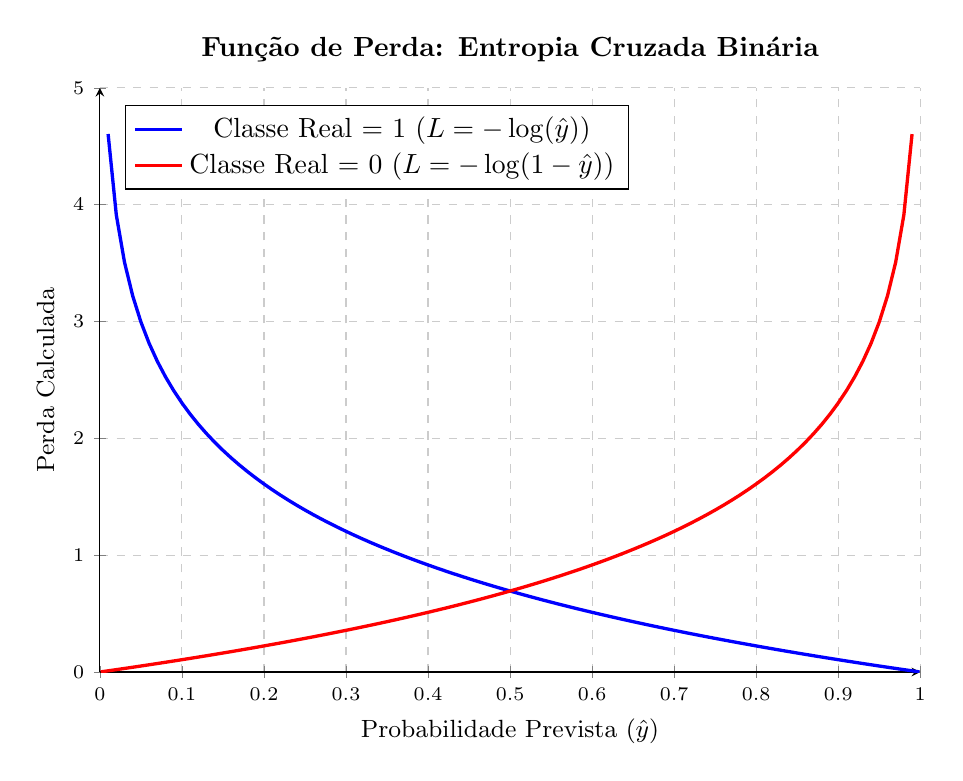
\begin{tikzpicture}
    \begin{axis}[
        title={Função de Perda: Entropia Cruzada Binária},
        xlabel={Probabilidade Prevista ($\hat{y}$)},
        ylabel={Perda Calculada},
        axis lines=left,              % Eixos no canto inferior esquerdo
        grid=major,                   % Adiciona uma grade principal
        grid style={dashed, gray!40},   % Estilo da grade
        xmin=0, xmax=1,               % Limites do eixo x
        ymin=0, ymax=5,               % Limites do eixo y
        legend pos=north west,      % Posição da legenda
        width=12cm,                   % Largura do gráfico
        height=9cm,                   % Altura do gráfico
        title style={font=\bfseries},
        label style={font=\small},
        tick label style={font=\scriptsize}
    ]
        % Curva para a classe real y=1
        \addplot[
            domain=0.01:0.999, % Domínio para evitar log(0)
            samples=100,
            color=blue,
            very thick
        ] {-ln(x)};
        \addlegendentry{Classe Real = 1 ($L = -\log(\hat{y})$)}

        % Curva para a classe real y=0
        \addplot[
            domain=0.001:0.99, % Domínio para evitar log(0)
            samples=100,
            color=red,
            very thick
        ] {-ln(1-x)};
        \addlegendentry{Classe Real = 0 ($L = -\log(1-\hat{y})$)}
        
    \end{axis}
\end{tikzpicture}

\begin{equacaodestaque}{Derivada da Entropia Cruzada Binária}
    \frac{\partial L}{\partial \hat{y}} = \frac{\hat{y} - y}{\hat{y}(1 - \hat{y})}
    \label{eq:binary-cross-entropy-derivada}
\end{equacaodestaque}

\subsection{Perda Hinge (Hinge Loss)}

\begin{equacaodestaque}{Hinge Loss}
    L(y, f(x)) = \max(0, 1 - y \cdot f(x))
    \label{eq:hinge-loss}
\end{equacaodestaque}

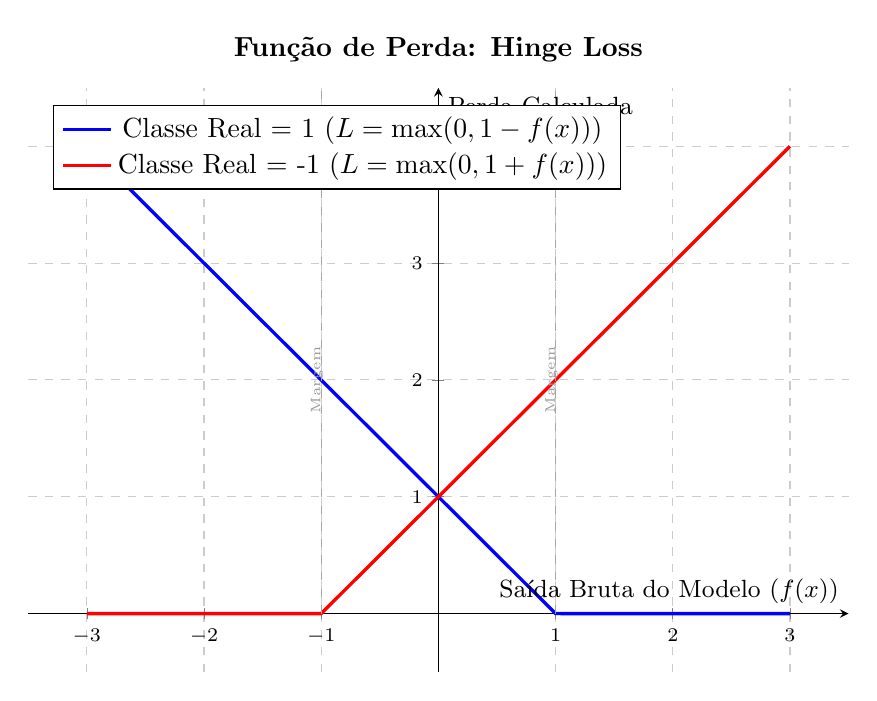
\begin{tikzpicture}
    \begin{axis}[
        title={Função de Perda: Hinge Loss},
        xlabel={Saída Bruta do Modelo ($f(x)$)},
        ylabel={Perda Calculada},
        axis lines=middle,          % Eixos centrados em (0,0)
        grid=major,                 % Adiciona uma grade principal
        grid style={dashed, gray!40}, % Estilo da grade
        xmin=-3.5, xmax=3.5,        % Limites do eixo x
        ymin=-0.5, ymax=4.5,         % Limites do eixo y
        legend pos=north west,      % Posição da legenda
        width=12cm,                 % Largura do gráfico
        height=9cm,                 % Altura do gráfico
        title style={font=\bfseries},
        label style={font=\small},
        tick label style={font=\scriptsize}
    ]
        % Curva para a classe real y=+1
        \addplot[
            domain=-3:3, 
            samples=100, 
            color=blue, 
            very thick
        ] {max(0, 1-x)};
        \addlegendentry{Classe Real = 1 ($L=\max(0, 1-f(x))$)}

        % Curva para a classe real y=-1
        \addplot[
            domain=-3:3, 
            samples=100, 
            color=red, 
            very thick
        ] {max(0, 1+x)};
        \addlegendentry{Classe Real = -1 ($L=\max(0, 1+f(x))$)}
        
        % Opcional: Linhas tracejadas para marcar as margens
        \draw[dashed, gray!70] (axis cs:1, 0) -- (axis cs:1, 4.5);
        \draw[dashed, gray!70] (axis cs:-1, 0) -- (axis cs:-1, 4.5);
        \node[above, gray!80, font=\tiny, rotate=90] at (axis cs:1.1, 2) {Margem};
        \node[above, gray!80, font=\tiny, rotate=90] at (axis cs:-0.9, 2) {Margem};
        
    \end{axis}
\end{tikzpicture}

\begin{equacaodestaque}{Derivada da Hinge Loss}
    \frac{\partial L}{\partial f(x)} = 
    \begin{cases} 
      -y & \text{se } y \cdot f(x) < 1 \\
      0 & \text{se } y \cdot f(x) \ge 1
    \end{cases}
    \label{eq:hinge-loss-derivada}
\end{equacaodestaque}

\section{Funções de Perda para Classificação Multilabel}

\subsection{Entropia Cruzada Categórica (Categorical Cross-Entropy)} 

\begin{equacaodestaque}{Entropia Cruzada Categórica}
    L(y, \hat{y}) = - \sum_{c=1}^{C} y_c \log(\hat{y}_c)
    \label{eq:categorical-cross-entropy}
\end{equacaodestaque}

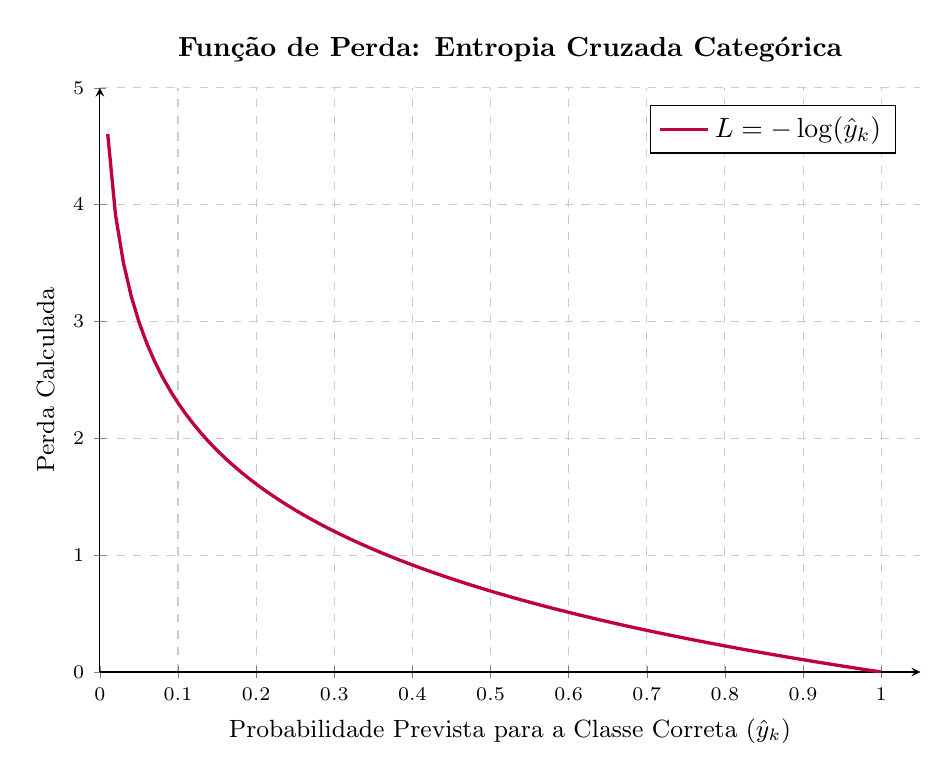
\begin{tikzpicture}
    \begin{axis}[
        title={Função de Perda: Entropia Cruzada Categórica},
        xlabel={Probabilidade Prevista para a Classe Correta ($\hat{y}_k$)},
        ylabel={Perda Calculada},
        axis lines=left,              % Eixos no canto inferior esquerdo
        grid=major,                   % Adiciona uma grade principal
        grid style={dashed, gray!40},   % Estilo da grade
        xmin=0, xmax=1.05,            % Limites do eixo x
        ymin=0, ymax=5,               % Limites do eixo y
        legend pos=north east,        % Posição da legenda
        width=12cm,                   % Largura do gráfico
        height=9cm,                   % Altura do gráfico
        title style={font=\bfseries},
        label style={font=\small},
        tick label style={font=\scriptsize}
    ]
        % Plota a função -log(y_k_hat)
        \addplot[
            domain=0.01:1, % Domínio para evitar log(0)
            samples=100,
            color=purple,
            very thick
        ] {-ln(x)};
        
        \addlegendentry{$L = -\log(\hat{y}_k)$}
        
    \end{axis}
\end{tikzpicture}

\begin{equacaodestaque}{Derivada da Entropia Cruzada Categórica}
    \frac{\partial L}{\partial z_i} = \hat{y}_i - y_i
    \label{eq:category-cross-entropy-derivada}
\end{equacaodestaque}

\subsection{Entropia Cruzada Categórica Esparsa (Sparse Categorical Cross-Entropy)}

\begin{equacaodestaque}{Entropia Cruzada Categórica Esparsa}
    L_i = - \log(\hat{y}_{i, y_i})
    \label{eq:sparse-categorical-cross-entropy}
\end{equacaodestaque}

\begin{equacaodestaque}{Derivada da Entropia Cruzada Categórica Esparsa}
    \frac{\partial L_i}{\partial z_{i,k}} = \hat{y}_{i,k} - y_{i,k}
    \label{eq:sparse-categorical-cross-entropy-derivada}
\end{equacaodestaque}

\section{Comparativo: Funções de Perda para Classificação}

\section{Fluxograma: Escolhendo a Função de Perda Ideal}